% ----------------------------------------------------------------
% MANG2023 Effective Business Performance Assignment.tex
% ---------------------------------------------------------------- 
\documentclass{ecsarticle}     % Use the Article Style
%\documentclass[review]{elsarticle}
\usepackage{natbib}            % Use Natbib style for the refs.
\graphicspath{./Figures/}
\usepackage{appendix}
\usepackage{color}
\usepackage{ transparent}
\usepackage{lipsum}
\usepackage[colorinlistoftodos]{todonotes}
\usepackage{multirow}
\usepackage{wrapfig}
\newcommand{\inote}[1] {\todo[inline]{#1}}
\def\citeapos#1{\citeauthor{#1}'s (\citeyear{#1})}
\removecolourlinks    % Uncomment this command to remove colour from any links
% ----------------------------------------------------------------
\begin{document}
\frontmatter
\title      {MANG6143 Project Risk Management}
\authors    {\texorpdfstring
             {\href{mailto:tjs1g10@ecs.soton.ac.uk}{Thomas J. Smith}}
             {Thomas J.Smith}
            }
\purpose  {}
\company       {MEng Electronic Engineering with Power Systems}
\addresses  {\purname\\\coname\\\univname}
\date       {\today}
\subject    {Performance Uncertainty Management Processes - PUMPs}
\keywords   {}
\maketitle
\begin{abstract}
%Knowledge and Understanding
%On successful completion of the unit you will be able to:
%\begin{itemize}
%\item discuss the usefulness of a variety of risk management frameworks,
%\item explain the problems associated with measuring performance,
%\item explain the problems associated with estimating probabilities,
%\item explain related ‘qualitative’ issues,
%\item understand the motives for undertaking formal risk management processes,
%\item be aware of limitations of some common practice,
%\item describe the issues to be addressed in establishing a formal process.
%\end{itemize}
%Subject Specific Intellectual Skills
%On successful completion of the unit you will be able to:
%\begin{itemize}
%\item discuss the application of a formal risk management process in a project context,  
%\item show how to identify an effective structure for addressing uncertainty, opportunity and risk associated with any project.
%\end{itemize}
%
%Key Skills
%By the end of the unit you will develop your ability in the following skills: 
%numeracy in terms of uncertainty, opportunity and risk, group working and communication during the module and subsequently through the assignment, key skills in information handling, critical analysis and written communication.

\end{abstract}


% -----------------------
% lstpatch.sty
% -----------------------
% lstpatch cannot be distributed with these files. I believe it is only needed if the
% \lstlistoflistings is used. So this has been turned off by default. Re-add if required:
% \usepackage{lstpatch}
% \lstlistoflistings
% You will need to download lstpatch, possibly from:
% http://web.mit.edu/texsrc/source/latex/listings/lstpatch.sty
% -----------------------

\mainmatter
%  Pt1.tex
% !TeX spellcheck = en_GB
% !TeX root = ProjectRiskManagement.tex

\section{The PUMP Approach to Uncertainty and Underlying Complexity Management}

%Introduction to risk and opportunity, underlying complexity. 

%Challenge of traditional view of risk.
The phrasing ``uncertainty and underlying complexity management'' has been specifically selected as the title of this section to contrast with the risk management title of the course as a whole.
Traditional views of risk management offer a limited scope and an incomplete picture.
Often the focus is event uncertainty reflecting the standard dictionary definition of risk: \textit{a hazard, chance of bad consequences, exposure to mischance} \citep{OED}.
This approach does not address the whole of the uncertainty affecting the project, and in the worst case can lead to failed delivery of project objectives.
The Performance Uncertainty Management Process (PUMP) framework encourages departure from the event-centric approach advocated by best practice, to consider all corporate, operational and planning sources of uncertainty.
This expanded perspective allows the capture of ambiguity uncertainty, inherent variability, systematic uncertainty, as well as event uncertainty.
Utilising the PUMP framework shifts the focus of risk management towards the achievement of opportunity efficiency and risk efficiency, through the vehicle of uncertainty management.

% execution and delivery strategy shaping phase of a project's life cycle
Procedures ensure consistency and quality is maintained throughout repeated applications.
A good procedure is designed to be simple, repeatable and transparent.
However, this cannot be a uniform approach.
Some high complexity, high uncertainty projects require sophisticated, tailored procedures.
The PUMP framework supports this concept through PUMP packs; a set of PUMPs tailored to specific projects and project lifecycle stages.
%Particularly, this paper focusses on PUMPs within the context of the execution and delivery (E\&D) strategy shaping stage.

\subsection{The Project Lifecycle Context}
%Project life cycle introduction.
A traditional four stage view of the asset/change lifecycle is a useful starting point to consider the scope of a project.
The four stages are conceptualize, planning, execution and delivery (E\&D) and Utilization.
As explained, effective uncertainty management requires a macro-view of the entire project to capture the different aspects of uncertainty.
This leads to an elaboration of the lifecycle to incorporate 12 stages, each emphasizing a different management purpose.
There is discussion as to the usefulness of such high clarity in the lifecycle, however it provokes in-depth consideration of all types of uncertainty \citep{Ward1995145}.
Both views are shown in figure \ref{Figure:Project_Lifecycle}.

\begin{figure}[!h]
  \centering
    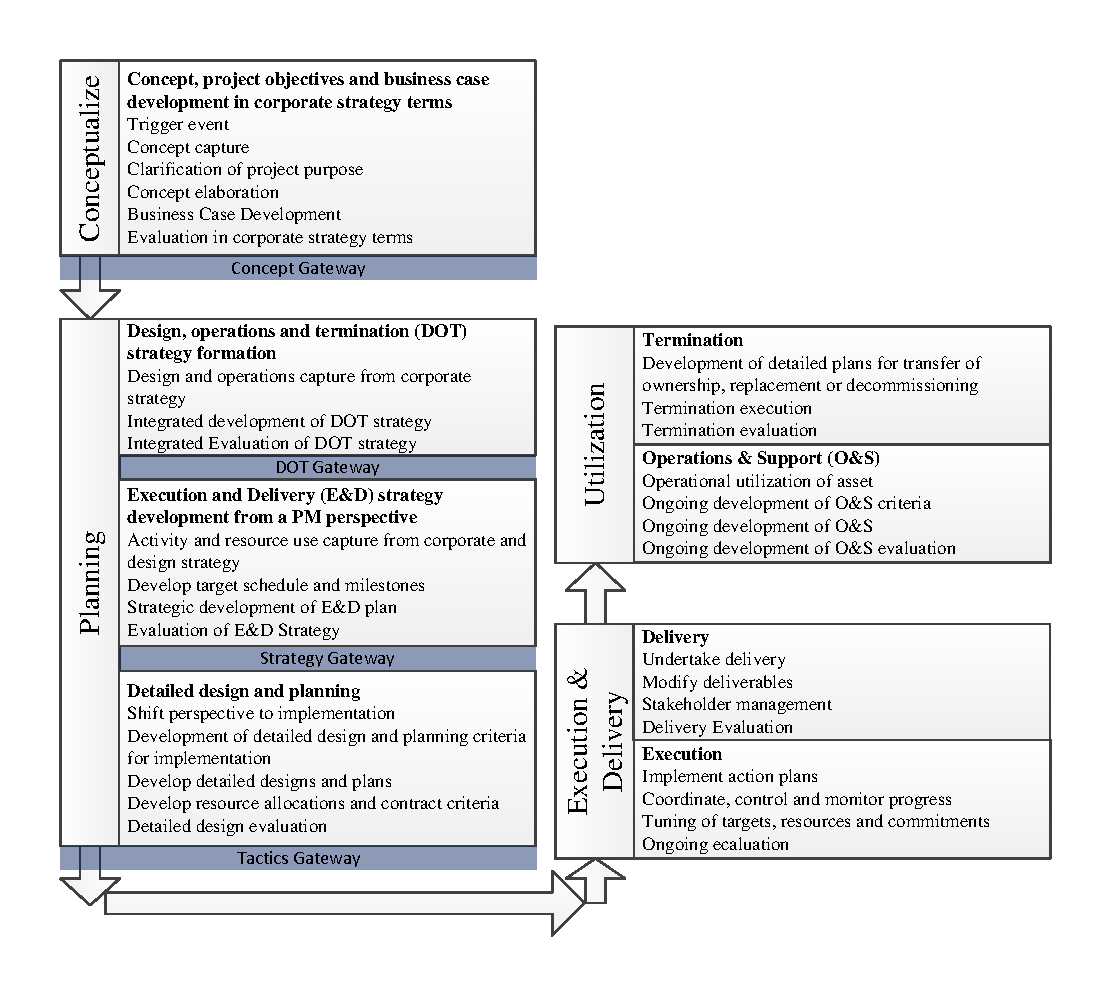
\includegraphics[width = \textwidth]{./Figures/ProjectLifecycleDetailedCurve.pdf} 
\caption{Twelve-stage asset/change lifecycle - adapted from \cite{chapman}}
\label{Figure:Project_Lifecycle}
\end{figure}

The planning stage of the traditional lifecycle is expanded to three shaping stages and three governance stages.
%The design, operations and termination (DOT) stage aims to derive a strategy for DOT from the corporate strategy developed in the conceptualize stage.
%A basic set of design criteria are built, and the objectives of the project are refined. 
%Integrated evaluation is important to ensure non-viable projects are halted before large expenditure.
The E\&D strategy shaping stage takes a form more familiar in traditional project management.
The activity and resource requirements are derived from the corporate strategy and the design, operations and termination (DOT) strategy. %DOT strategy.
This stage considers aspects of the project execution and asks how the asset/change will be delivered?
Schedule derivation takes place in the E\&D stage, including the reconciliation of corporate expectation and real-world plausibility.
%Again, integrated evaluation is vital to ensuring only viable projects proceed to later more expensive stages of the lifecycle.
Integrated evaluation is vital to ensuring only viable projects proceed to later more expensive stages of the lifecycle.
This paper is concerned with PUMPs tailored to this lifecycle stage.



\subsection{PUMP Overview}
%Explain concisely in your own words what you believe are the key overall features of a PUMP approach to project risk management in the execution and delivery strategy shaping phase of a project’s lifecycle. Compare these features with the PMI PIMBOK approach or any other form of common practice you are familiar with if you find this helpful, but focus on the PUMP approach. Use examples to illustrate your discussion if you wish, but concentrate on concepts and principles. This will be a largely descriptive summary of your interpretation of the lectures and associated reading. It will demonstrate your grasp of the central core of the unit’s material as a whole, and should be approached with a view to demonstrating this understanding..

The PUMP approach was developed through the assimilation of other industrial risk processes, building upon the best practice approaches from project management bodies.
The process was developed by Acres International Management Services for BP and first implemented on the Magnus offshore North Sea project in 1976. 
\citet{SCERT} published the process as SCERT (Synergistic Contingency Evaluation and Review Technique) and the technique has since been used in a variety of high profile projects for BP, National Power and the Highways Agency.
The process has been refined and assimilated into a complete framework suitable for a variety of clarity requirements.


The PUMP process is a seven stage iterative cycle as shown in figure \ref{Figure:Project_Lifecycle}. 
A linear `right first time' approach is not a clarity efficient methodology.
A version of Pareto's principle, sometimes called the 80:20 rule \citep{Pareto1992}, empirically states that 20\% of the issues causes 80\% of the problems. 
The first iteration of the PUMP is a high level sweep to identify the key areas of concern.
Subsequent iterations focus on these issues until a sufficient level of clarity is achieved.
This allows the achievement of clarity efficiency, by minimising time spent on unnecessary detail while achieving the required level of understanding.

\begin{figure}[!h]
  \centering
\subfigure[Flowchart Visualisation]{
    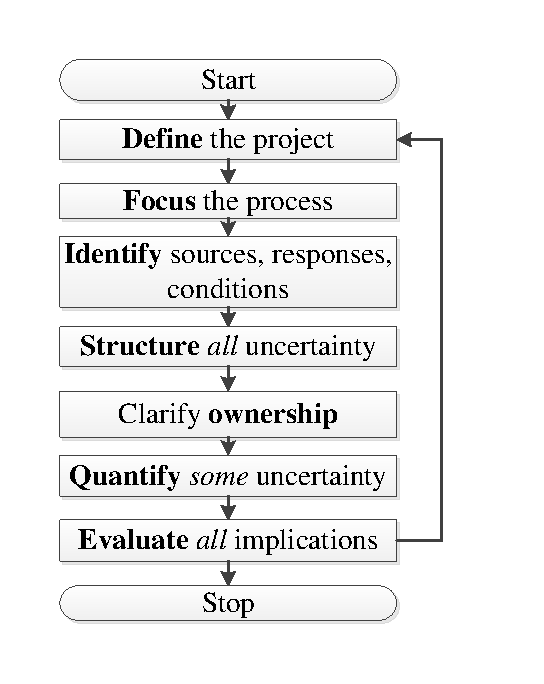
\includegraphics[height = 6cm]{./Figures/PUMPgeneric.pdf} 
	\label{Figure:GenericPUMP_Flow}
   } \quad
\subfigure[Gantt Chart Visualisation]{
    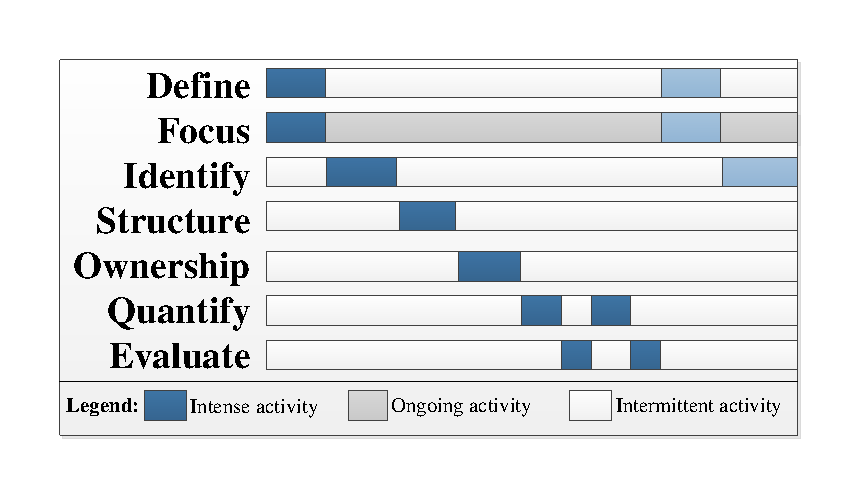
\includegraphics[height = 5cm]{./Figures/PUMPgenericGantt.pdf} 
	\label{Figure:GenericPUMP_Gantt}
   }
\caption{The generic PUMP process - adapted from \cite{chapman}}
\label{Figure:GenericPUMP_Both}
\end{figure}

The initiating phase of the generic PUMP is the \textbf{define} phase.
This phase defines and develops an understanding of the project as a basis to ask the right questions in subsequent phases.
It features high level context capture and approach development at a strategic level.
There are two key activities in this phase; consolidate and elaborate as shown in figure \ref{Figure:Define}.
A useful framework for adequately addressing these issues is the 7W's: where, who, why, what, whichway, wherewithal, when? 
Using the 7W's to consolidate the existing information, then sub-iterating in order to sufficiently define the project is a useful method to complete this phase.
The phase is complete when the project deliverables are fit for purpose.

The \textbf{focus} phase involves scoping the level of analysis required during the E\&D shaping lifecycle stage.
During this phase, the generic PUMP is tailored to the specific requirements of the project at hand as captured from the corporate context.
This phase is closely coupled with the define phase.
The aim is to achieve clarity efficiency by stating all working assumptions at an early stage.
The phase ends when the scope, strategy and plan for the tailored PUMP process is fit for purpose.

\begin{figure}[!h]
  \centering
\subfigure[Define Phase Process]{
    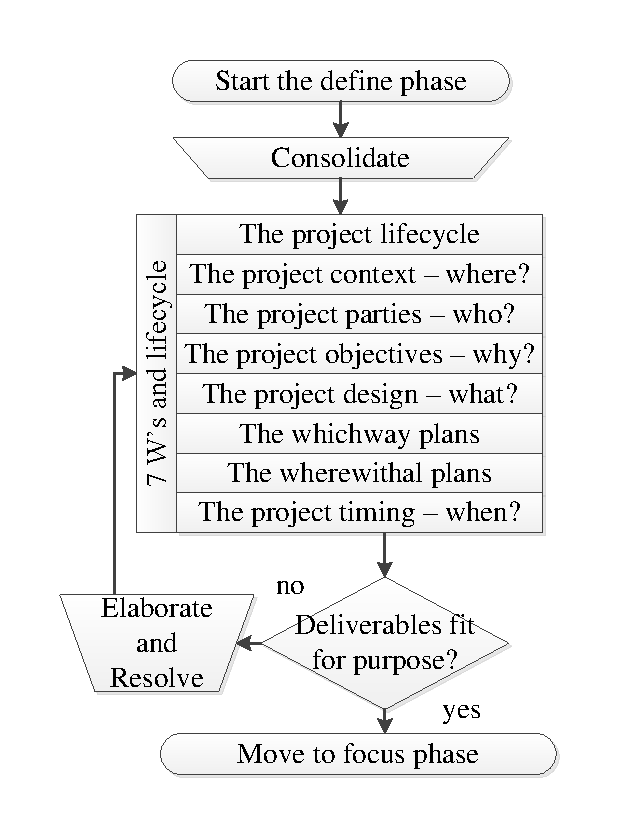
\includegraphics[height = 8cm]{./Figures/Define.pdf} 
	\label{Figure:Define}
   } \quad
\subfigure[Focus Phase Process]{
    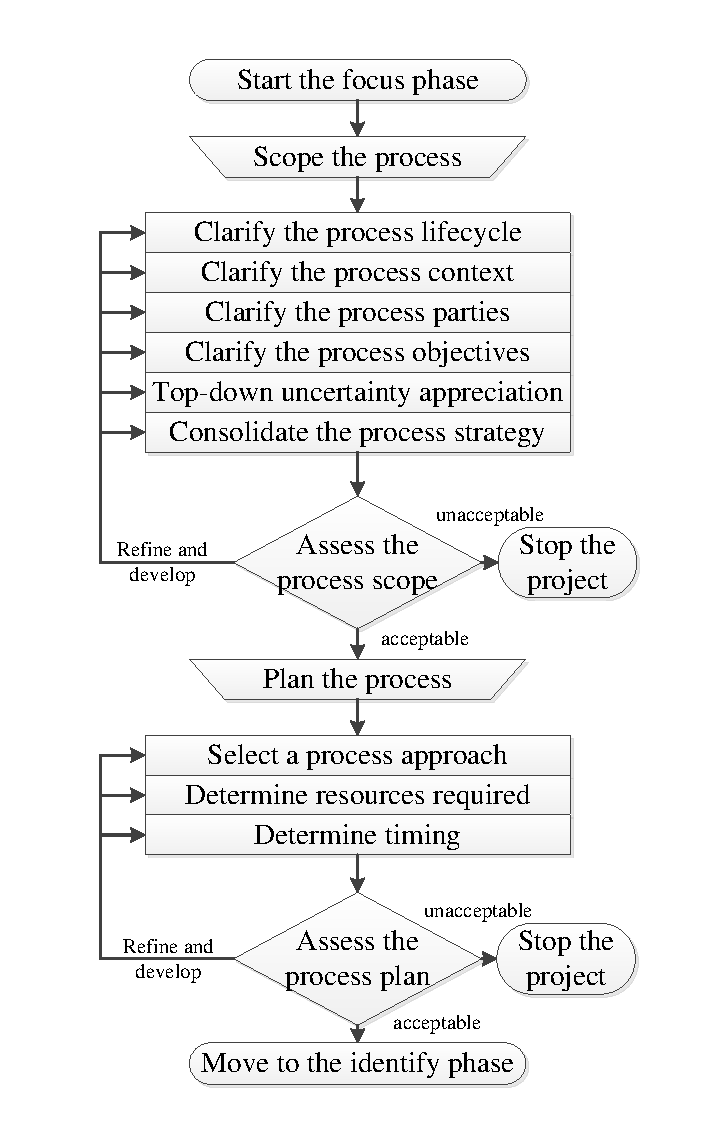
\includegraphics[height = 9.3cm]{./Figures/Focus.pdf} 
	\label{Figure:Focus}
   }
\caption{Phase process flowcharts - adapted from \cite{chapman}}
\label{Figure:DefineFocus}
\end{figure}

The identification of all sources of uncertainty, relevant response options and conditions is undertaken in the \textbf{identify} phase.
This phase has key distinguishing features that are vital to achieve clarity efficiency and to understand all relevant uncertainty and underlying complexity.
This is considered in detail in section \ref{s:Identify}.

Following the identification of sources of uncertainty, responses and conditions, an understanding of their relative importance is qualitatively established in the \textbf{structure} phase.
This phase contributes to the clarity efficient nature of PUMPs, by maximising the effort expended on issues of perceived importance.
Responses should also be considered, as early identification of powerful general responses means less effort is required to deal with specific responses.
Source-response diagrams, decision tress and influence diagrams are all useful tools for this purpose.
%\inote{Source-response p215 / faulttree chapman1979/ influencediagram p229}
Failure to deal with underlying complexity, assumptions, interdependencies and detail in this phase could endanger the success of the project.
Seemingly small details missed in the structure phase represent systematic uncertainty that could lead to later threats or missed opportunities.
Other key activities are shown in figure \ref{Figure:Structure}.

\begin{figure}[!h]
  \centering
    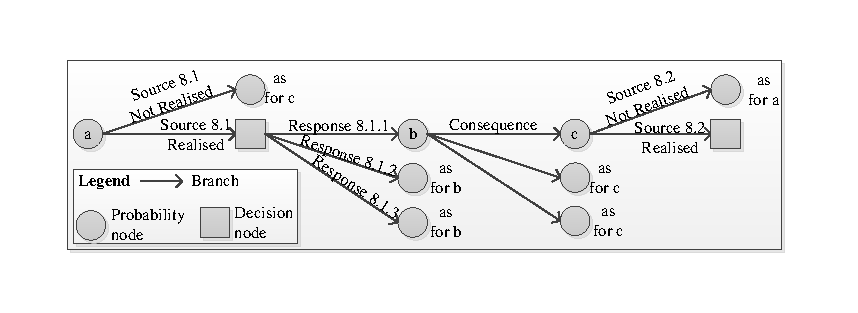
\includegraphics[height = 2.95cm]{./Figures/DecisionTreeChapman79.pdf} 
\caption{Partial Example probability/decision tree - adapted from \cite{SCERT}}
\label{Figure:Decisiontree}
\end{figure}

\begin{figure}[!h]
  \centering
    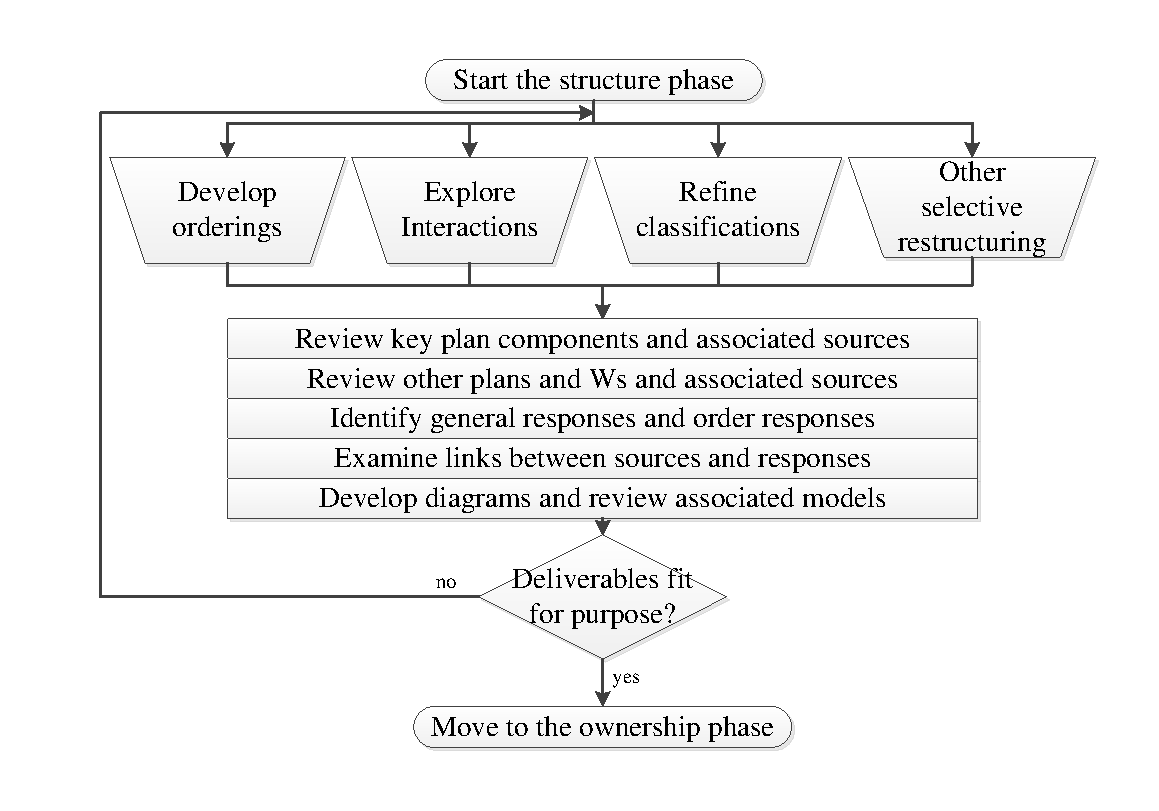
\includegraphics[width = 0.7\textwidth]{./Figures/Structure.pdf} 
\caption{Structure Phase Process - adapted from \cite{chapman}}
\label{Figure:Structure}
\end{figure}

%\begin{figure}[!h]
%  \centering
%\subfigure[Define Phase Process]{
%    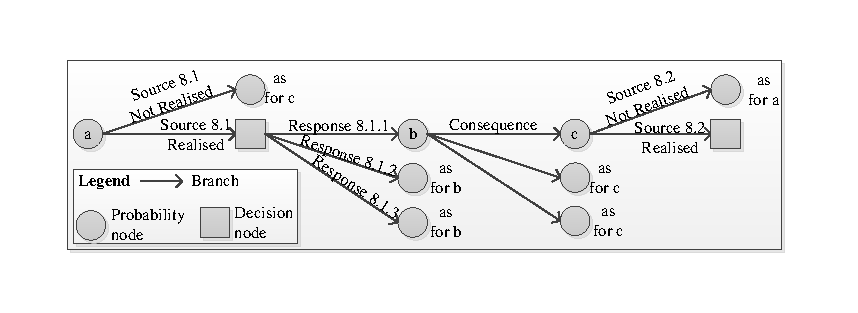
\includegraphics[height = 2cm]{./Figures/DecisionTreeChapman79.pdf} 
%	\label{Figure:Define}
%   } \quad
%\subfigure[Focus Phase Process]{
%    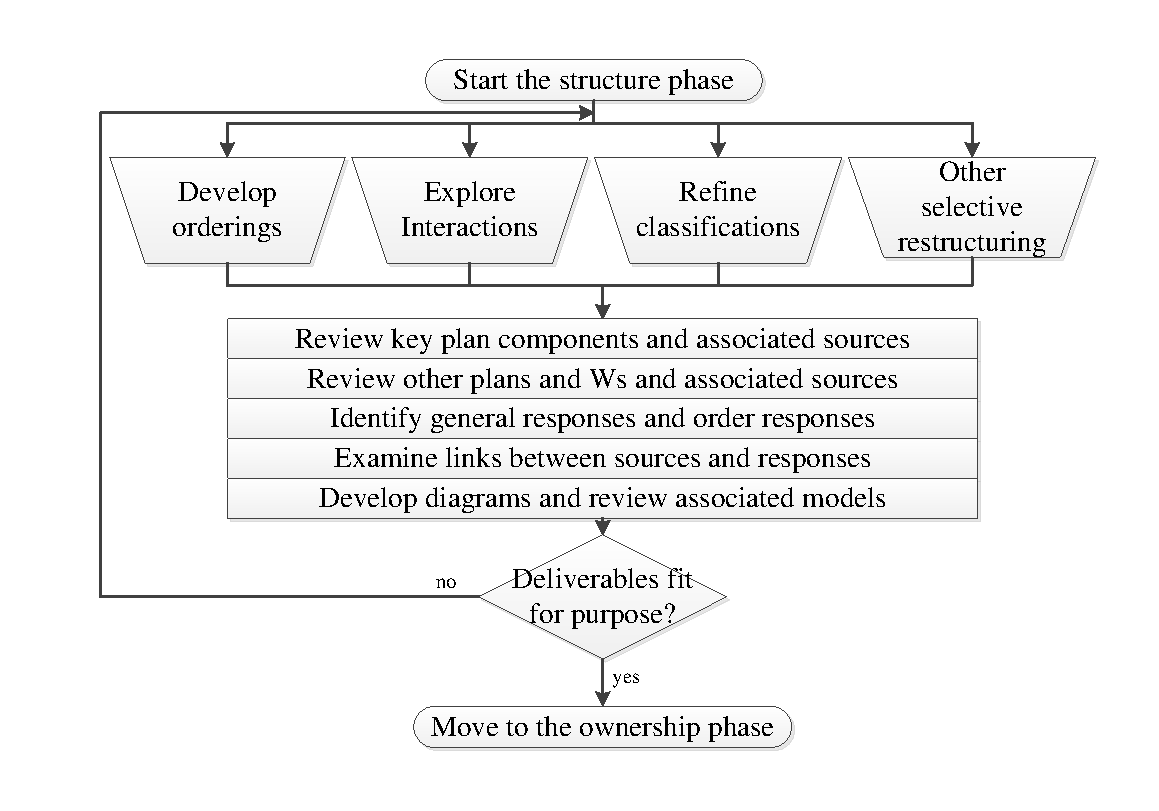
\includegraphics[height = 10cm]{./Figures/Structure.pdf} 
%	\label{Figure:Focus}
%   }
%\caption{Phase process flowcharts - adapted from \cite{chapman}}
%\label{Figure:DefineFocus}
%\end{figure}

The clarify \textbf{ownership} phase allocates financial and managerial responsibility for relevant sources of uncertainty.
In reality, all sources are allocated to a party whether explicitly or by default.
The key activities of this stage include developing a contracting strategy, distinguishing ownership and allocating responsibility.
The aim of the phase is a win-win outcome for all contractual parties, so that client and contractor objectives are aligned.
\inote{structure and ownership p238 visio diagrams required}

%The key deliverables of \textbf{Quantify}
%\inote{Quantify phase flowchart required}
The key deliverable of the \textbf{Quantify} phase is an informed basis for making critical project decisions in the pursuit of opportunity efficiency.
Clarity efficiency is achieved by sizing the data on the first iteration and decomposing to subsequent levels of detail where necessary in further iterations.
Probability Impact Grid (PIG) approaches widespread in industry and advocated by best practice.
PIGs suffer from subjective interpretation of measuring terms as shown in \citet{Merkhofer}, a failure to address uncertainty of other than event uncertainty and granular quantisation of sources \citep{Cox2008}.
Where objective data is available, probabilistic density functions should be utilised.
It would be foolish to disregard the expertise of experienced personnel; hence where objective data is unavailable, subjective probabilities could be used.
The SRI technique published by \citet{spetzer} provides a framework for probability elicitation.
There are some complexities discussed by \citet{Merkhofer}, including strategic misrepresentation \citep{flyvbjerg} and it remains an inexact science.

\begin{figure}[!h]
  \centering
\subfigure[Example 5x5 Pig Approach - adapted from \cite{Cox2008}]{
    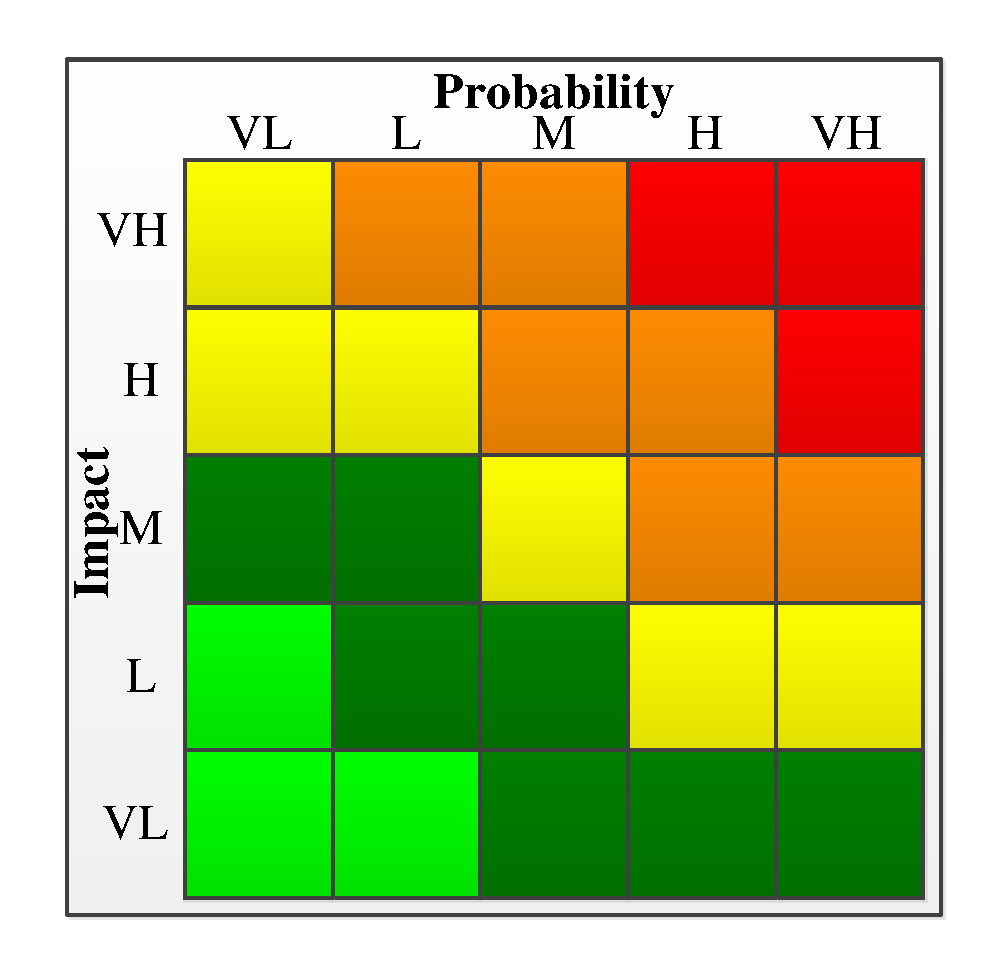
\includegraphics[height = 6cm]{./Figures/PIGCox.pdf} 
	\label{Figure:PIG}
   } \quad
\subfigure[Example Methods of Portraying Probability Density Functions - adapted from \cite{chapman}]{
    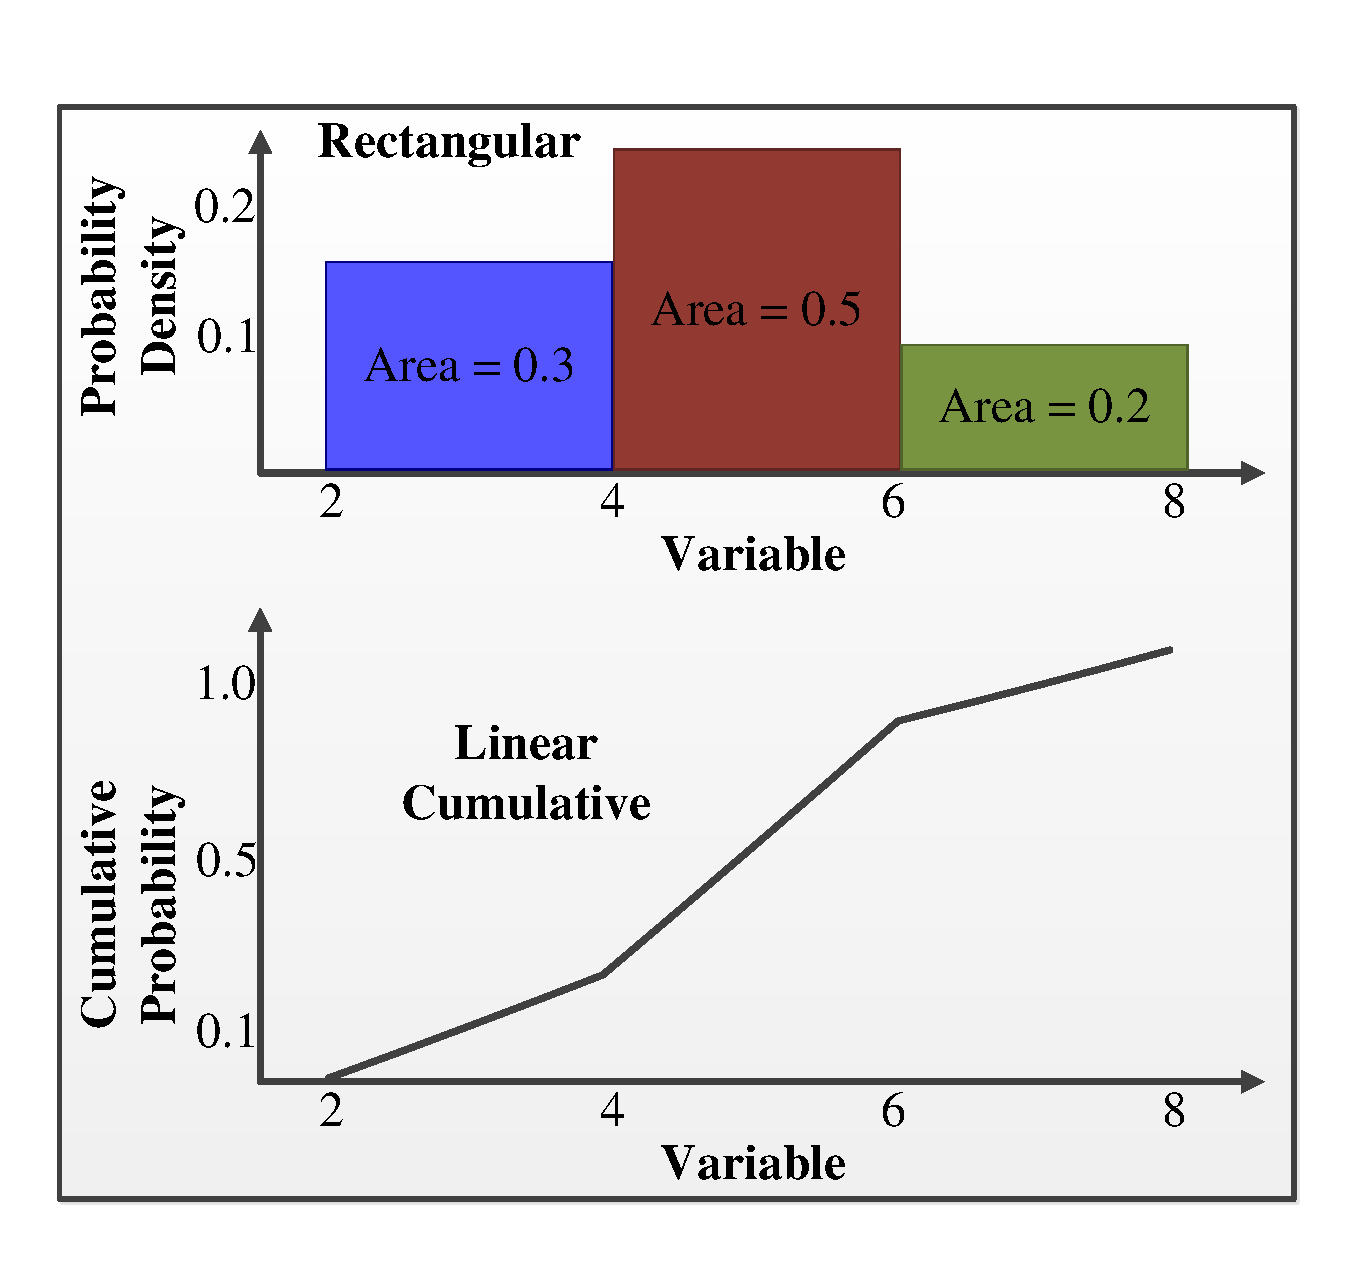
\includegraphics[height = 6cm]{./Figures/Hist.pdf} 
	\label{Figure:Hist}
   }
\caption{Potential Approaches to the Quantification of Data}
\label{Figure:DefineFocus}
\end{figure}


The \textbf{evaluate} phase involves synthesizing the results of the quantify phase and assessing the statistical significance of results.
This phase is critical to the successful application of the PUMP process, and consolidates much of the understanding of uncertainty.
This phase is considered in detail in section \ref{s:Evaluate}.


\subsection{The Clarity Efficient Approach to Opportunity Efficiency}
This section has given a brief overview of a high clarity PUMP for the E\&D strategy shaping phase, except for the identify and evaluate phases considered later.
Several recurring themes throughout all PUMP phases have been illustrated including the pursuit of clarity efficiency, flexibility and a holistic approach to uncertainty management.
The following sections will consider the Identify and Evaluate phases in detail.


%1200words.
\section{Identification of Uncertainty}
For the identify phase of the PUMP approach, in the execution and delivery strategy shaping phase of a project’s lifecycle, explain concisely in your own words what you believe are the key features of a PUMP approach, comparing these features with the PMI PIMBOK approach or any other form of common practice you are familiar with. Your discussion should demonstrate your ability to understand a particular area of the course material in depth, based on selective reading, critical analysis and the case study exercise. Use examples to illustrate your discussion if you wish, making use of the Samdo case study if you wish, but concentrate on concepts and principles. Build on your Part 1 answer, avoiding repetition of earlier discussion.
900words.

%  Pt3.tex
% !TeX spellcheck = en_GB
% !TeX root = ProjectRiskManagement.tex
\section{Evaluate \textit{All} the Relevant Implications} \label{s:Evaluate}

%For the evaluate phase of the PUMP approach, in the execution and delivery strategy shaping phase of a project’s lifecycle, explain concisely in your own words what you believe are the key features of a PUMP approach, comparing these features with the PMI PIMBOK approach or any other form of common practice you are familiar with. Your discussion should demonstrate your ability to understand a particular area of the course material in depth, based on selective reading, critical analysis and the case study exercise. Use examples to illustrate your discussion if you wish, and make use of the Transcon case study if you wish, but concentrate on concepts and principles. Build on your Parts 1 and 2 answers, avoiding repetition.

%900 words.

The evaluate phase is the pivotal phase of the PUMP process and plays a critical role in consolidating understanding and controlling PUMP iterations.
The phase involves collating all of the insight and results gained during previous phases into a coherent and comprehensive narrative understanding of the uncertainty involved and the response options available in a clarity efficient manner.
An intuitive understanding of statistical and causal dependence is required to adequately understand the implications of underlying, often-complex relationships.
Following result synthesis, the results must be presented in the most clarity efficient format, usually using diagrams, to allow interpretation of their practical meaning.
This section is not a complete summary of the evaluate phase, but considers some of the tools available for efficient delivery of the phase objectives in some detail, with further areas of consideration in \cite{chapman}.

The phase deliverables may be a simple list of priority sources and responses at early project stages.
This may be developed further to diagnose issues and suggest revisions to base plans so that specific sources of risk inefficiency are avoided and to ensure opportunities are captured.
There are five `modes' of operation of the phase, shown in figure \ref{Figure:Evaluate}.

\begin{figure}[!h]
  \centering
    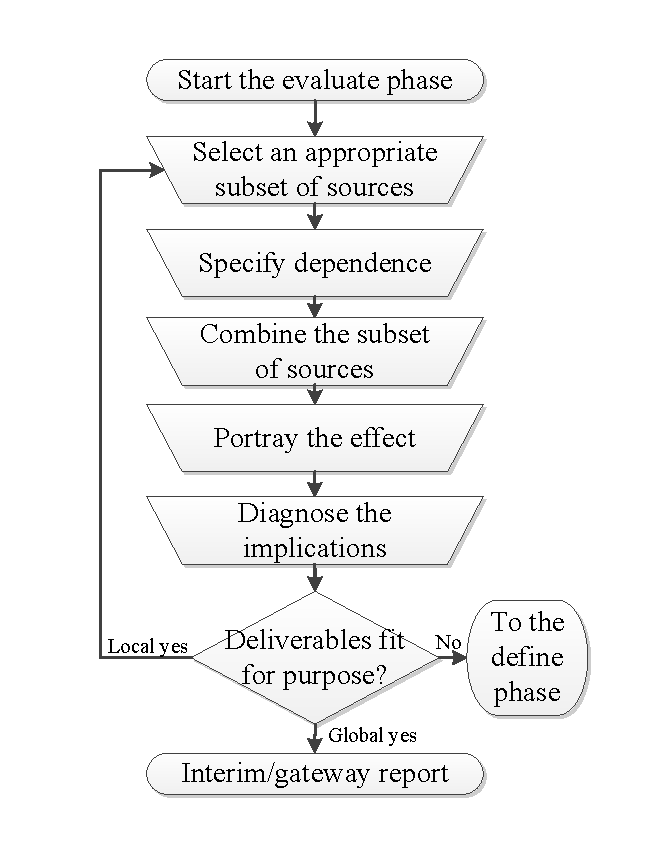
\includegraphics[width = 0.42\textwidth]{./Figures/Evaluate.pdf} 
\caption{Evaluate phase process - adapted from \cite{chapman}}
\label{Figure:Evaluate}
\end{figure}

Specifying dependence is an important mode of the phase.
To simplify the approach, many practioners following common processes may assume independence between sources.
This is an extremely dangerous approach, and any formal analysis based on this assumption on a non-evidential basis should be immediately discounted.
Falsely assuming independence paints an optimistic picture of the circumstances by ignoring the knock-on effects of underlying complexity.
This can be compounded by over-simplified computational tools that aim to make calculations easier, and by a managerial preference for limited variability. 
Positive dependence is a more reasonable assumption, making a more conservative, robust assessment of the impacts. 
In high-clarity contexts, complex statistical and causal dependencies may require more sophisticated modelling approaches to adequately understand the full implications.

The dangers of making false dependency assumptions is shown in the contrast between independent and positive dependence in figure \ref{Figure:ImpactsDependence}.
Two identical probability functions are combined by addition, showing the difference caused by dependence assumptions.
Any dependence relation between 0-100\% can be achieved by linear interpolation between the two curves.

\begin{figure}[!h]
  \centering
\subfigure[$C_{a}$ and $C_{b}$ probability density functions are identical]{
    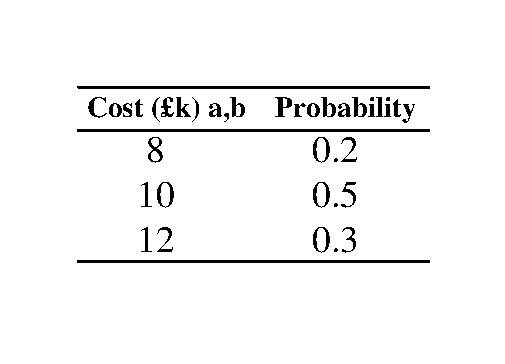
\includegraphics[width = 0.22\textwidth]{./Figures/Costabtab.pdf}
	\label{Table:DepValsab}
   }
\subfigure[$C_{i} = C_{a} + C_{b}$ probability density function assuming independence]{
    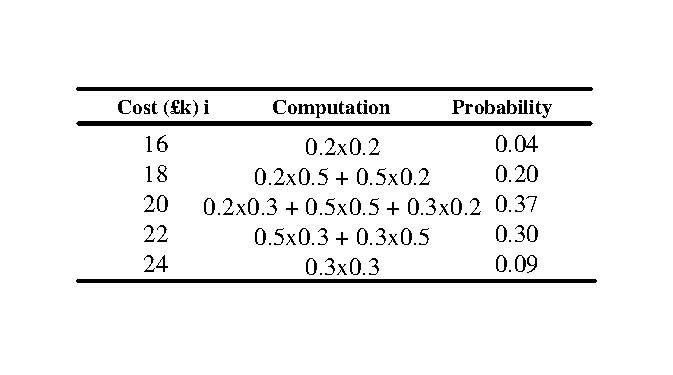
\includegraphics[width = 0.3\textwidth]{./Figures/Costitab.pdf}
	\label{Table:DepValsi}
   }
\subfigure[$C_{p} = C_{a} + C_{b}$ probability density function assuming positive dependence]{
    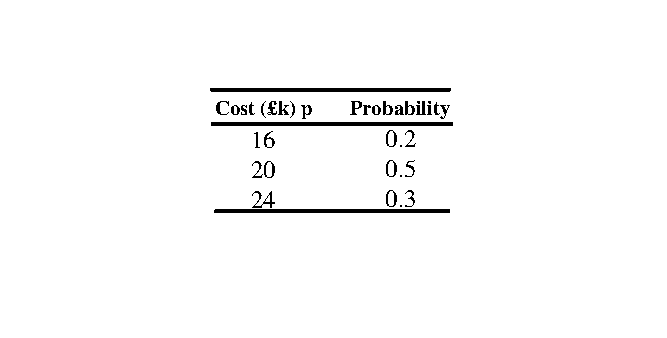
\includegraphics[width = 0.22\textwidth]{./Figures/Costptab.pdf}
	\label{Table:DepValsp}
   }

\subfigure[Cumulative probability distributions for the addition of $C_{a}$ and $C_{b}$]{
    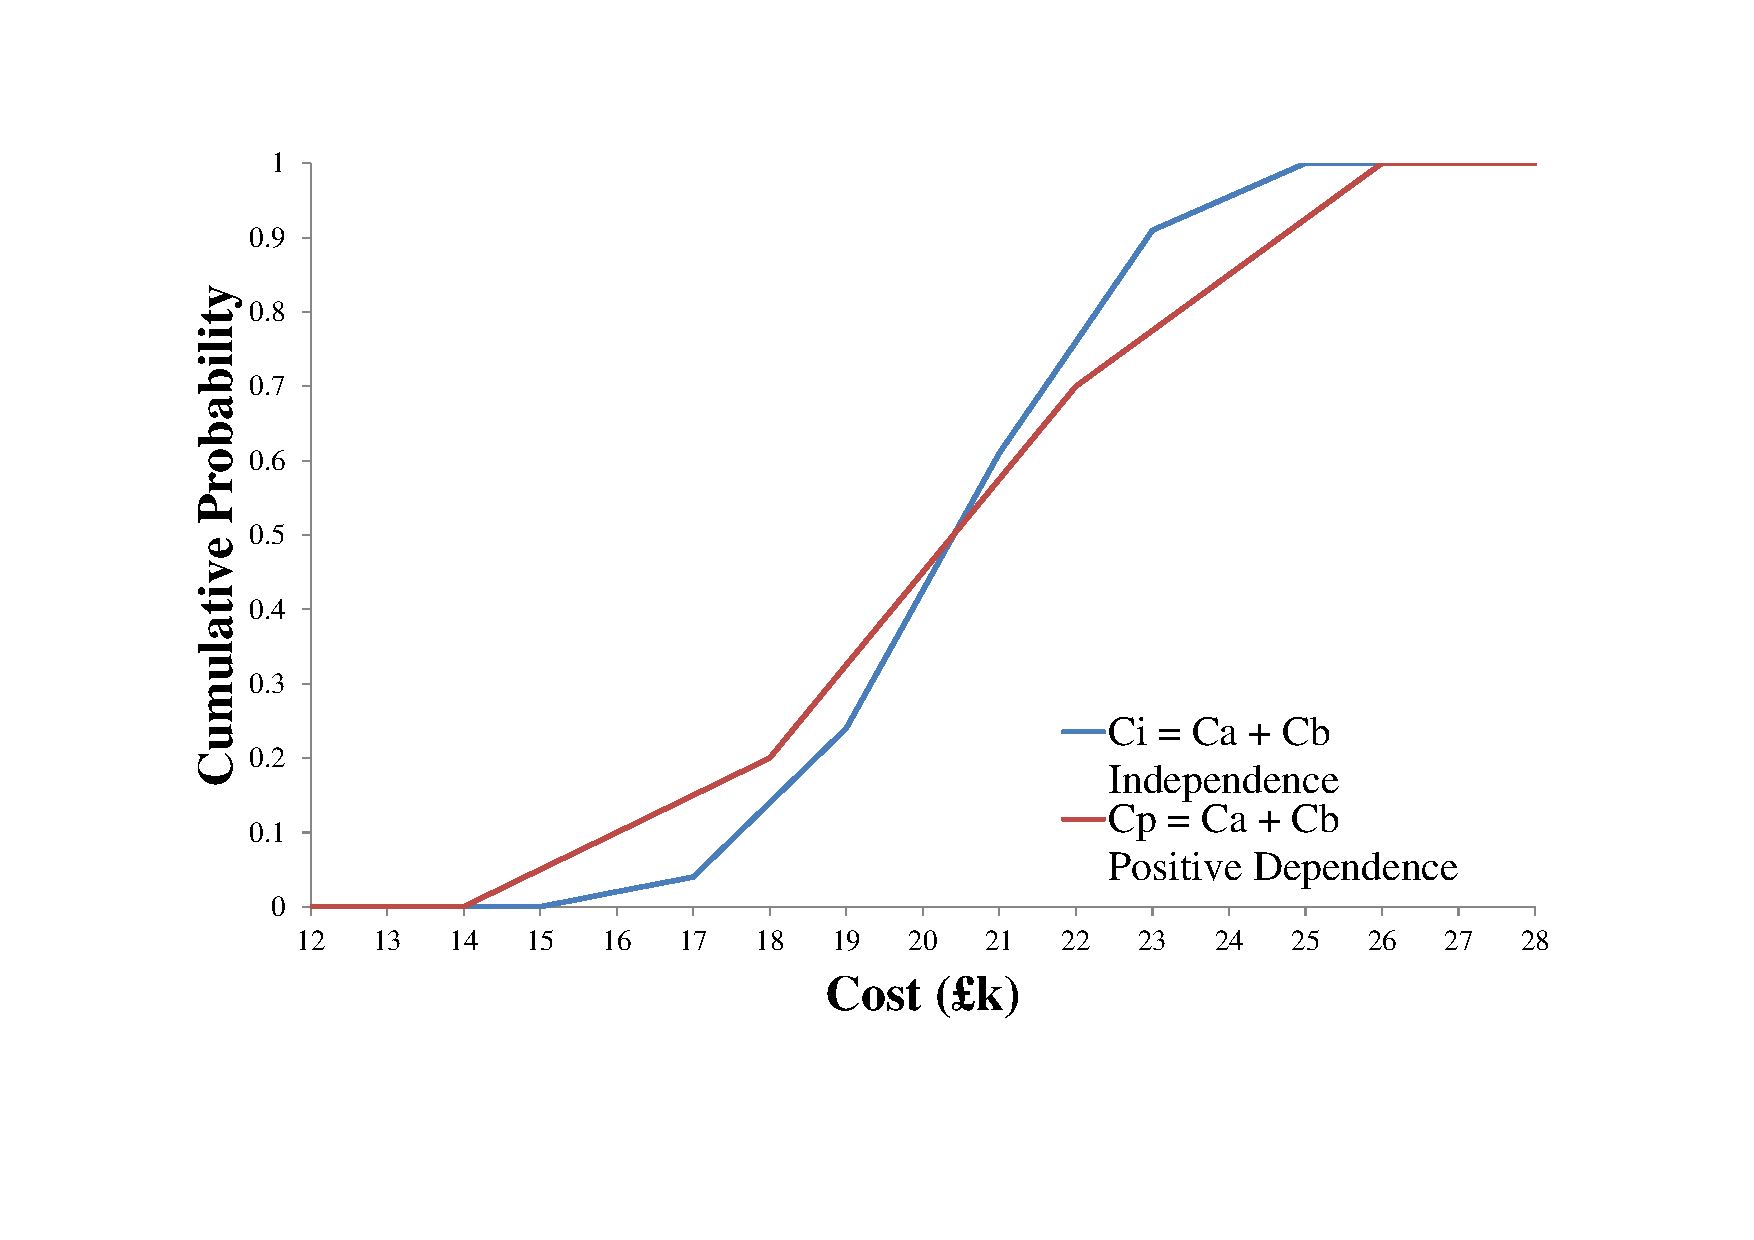
\includegraphics[width = 0.62\textwidth]{./Figures/Dependence.pdf} 
	\label{Figure:Dependency}
   }
\caption{The impacts of independence and positive dependence assumptions - adapted from \cite{chapman}}
\label{Figure:ImpactsDependence}
\end{figure}

Another key mode of the phase is to portray the effects. 
The story that has been developed throughout the analysis must be conveyed in the most clarity efficient manner to be of any practical value to the project organisation.
Sensitivity diagrams are an important tool for conveying and explaining uncertainty.
The common phrase ``a picture is worth a thousand words'' is relevant here.
A sensitivity diagram gives the audience the required information in a non-threatening easy-to-grasp format so that interpretation can take place and issues raised can be resolved.

The sensitivity diagram in figure \ref{Figure:SensDiag} shows the collation of six sources associated with a geotechnical investigation project in preparation for the construction of a power station.
A diagram of this type may be required for each activity in a network.
The gap between each curve portrays the effect of the labelled source.
The final source ``personnel availability for processing'' is clearly the most important source in this example, and more effort can be given to addressing this as required. 
The ordering of the sources are important, so that any causal and statistical dependence is portrayed by adjacency of sources.
A maximum of around six sources should be displayed on the diagram to ensure the meaning remains clear.
Less important sources can be combined so that only the most relevant aspects of the story are shown.

\begin{figure}[!h]
  \centering
    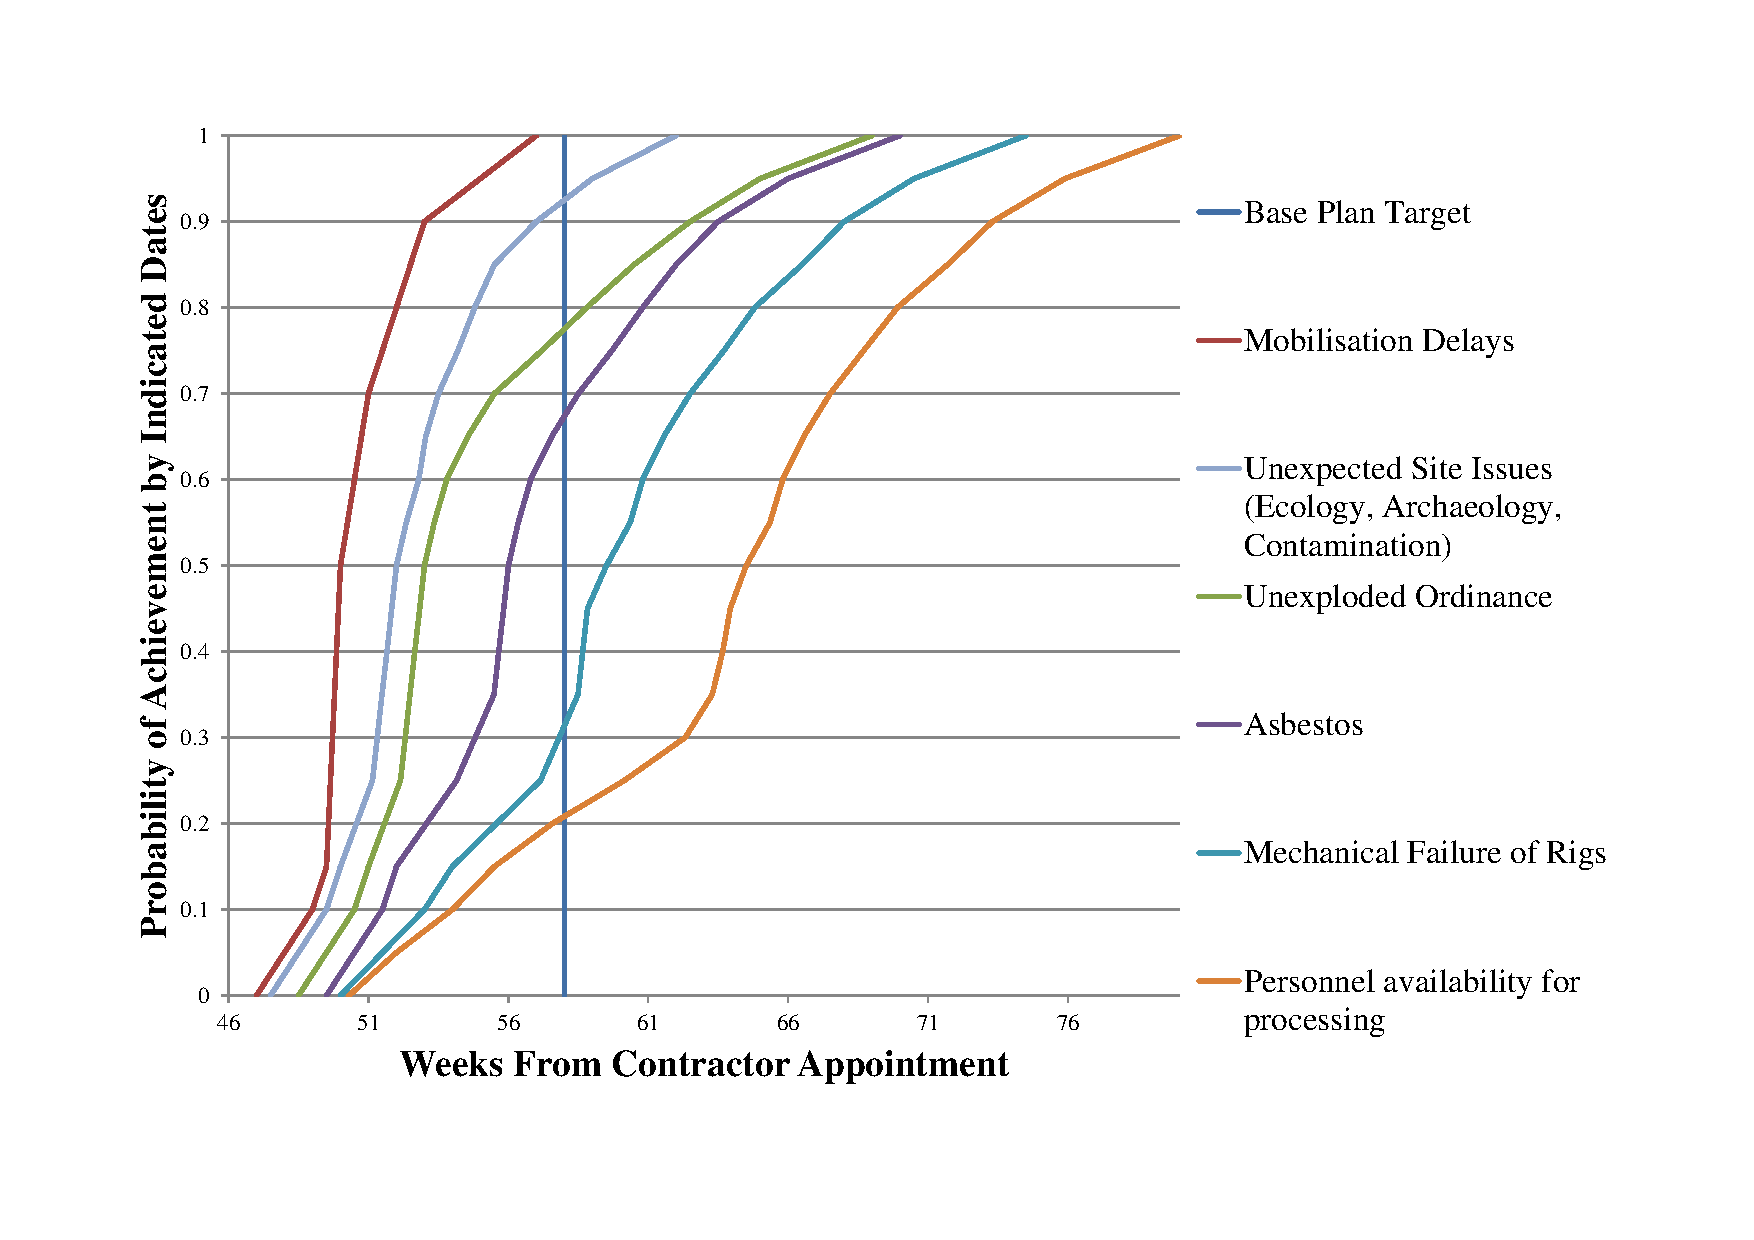
\includegraphics[width = 0.79\textwidth]{./Figures/Sensitivity_Diagram.pdf} 
\caption{Sensitivity diagram for geotechnical investigations completion date - adapted from \cite{chapman} \& \cite{hopkinson2008}}
\label{Figure:SensDiag}
\end{figure}

It may be useful to expand a sensitivity diagram where schedules are concerned. 
This can help develop a project strategy that includes realistic milestones and help identify contingency requirements \citep{hopkinson2008}.
Uncertainty can be decomposed through a number of project milestones and contracting activities, as in figure \ref{Figure:SensDiagGantt}.
This can be displayed alongside a Gantt chart to portray the schedule implications if this adds to understanding \citep{hopkinson2008}.

\begin{figure}[!h]
  \centering
    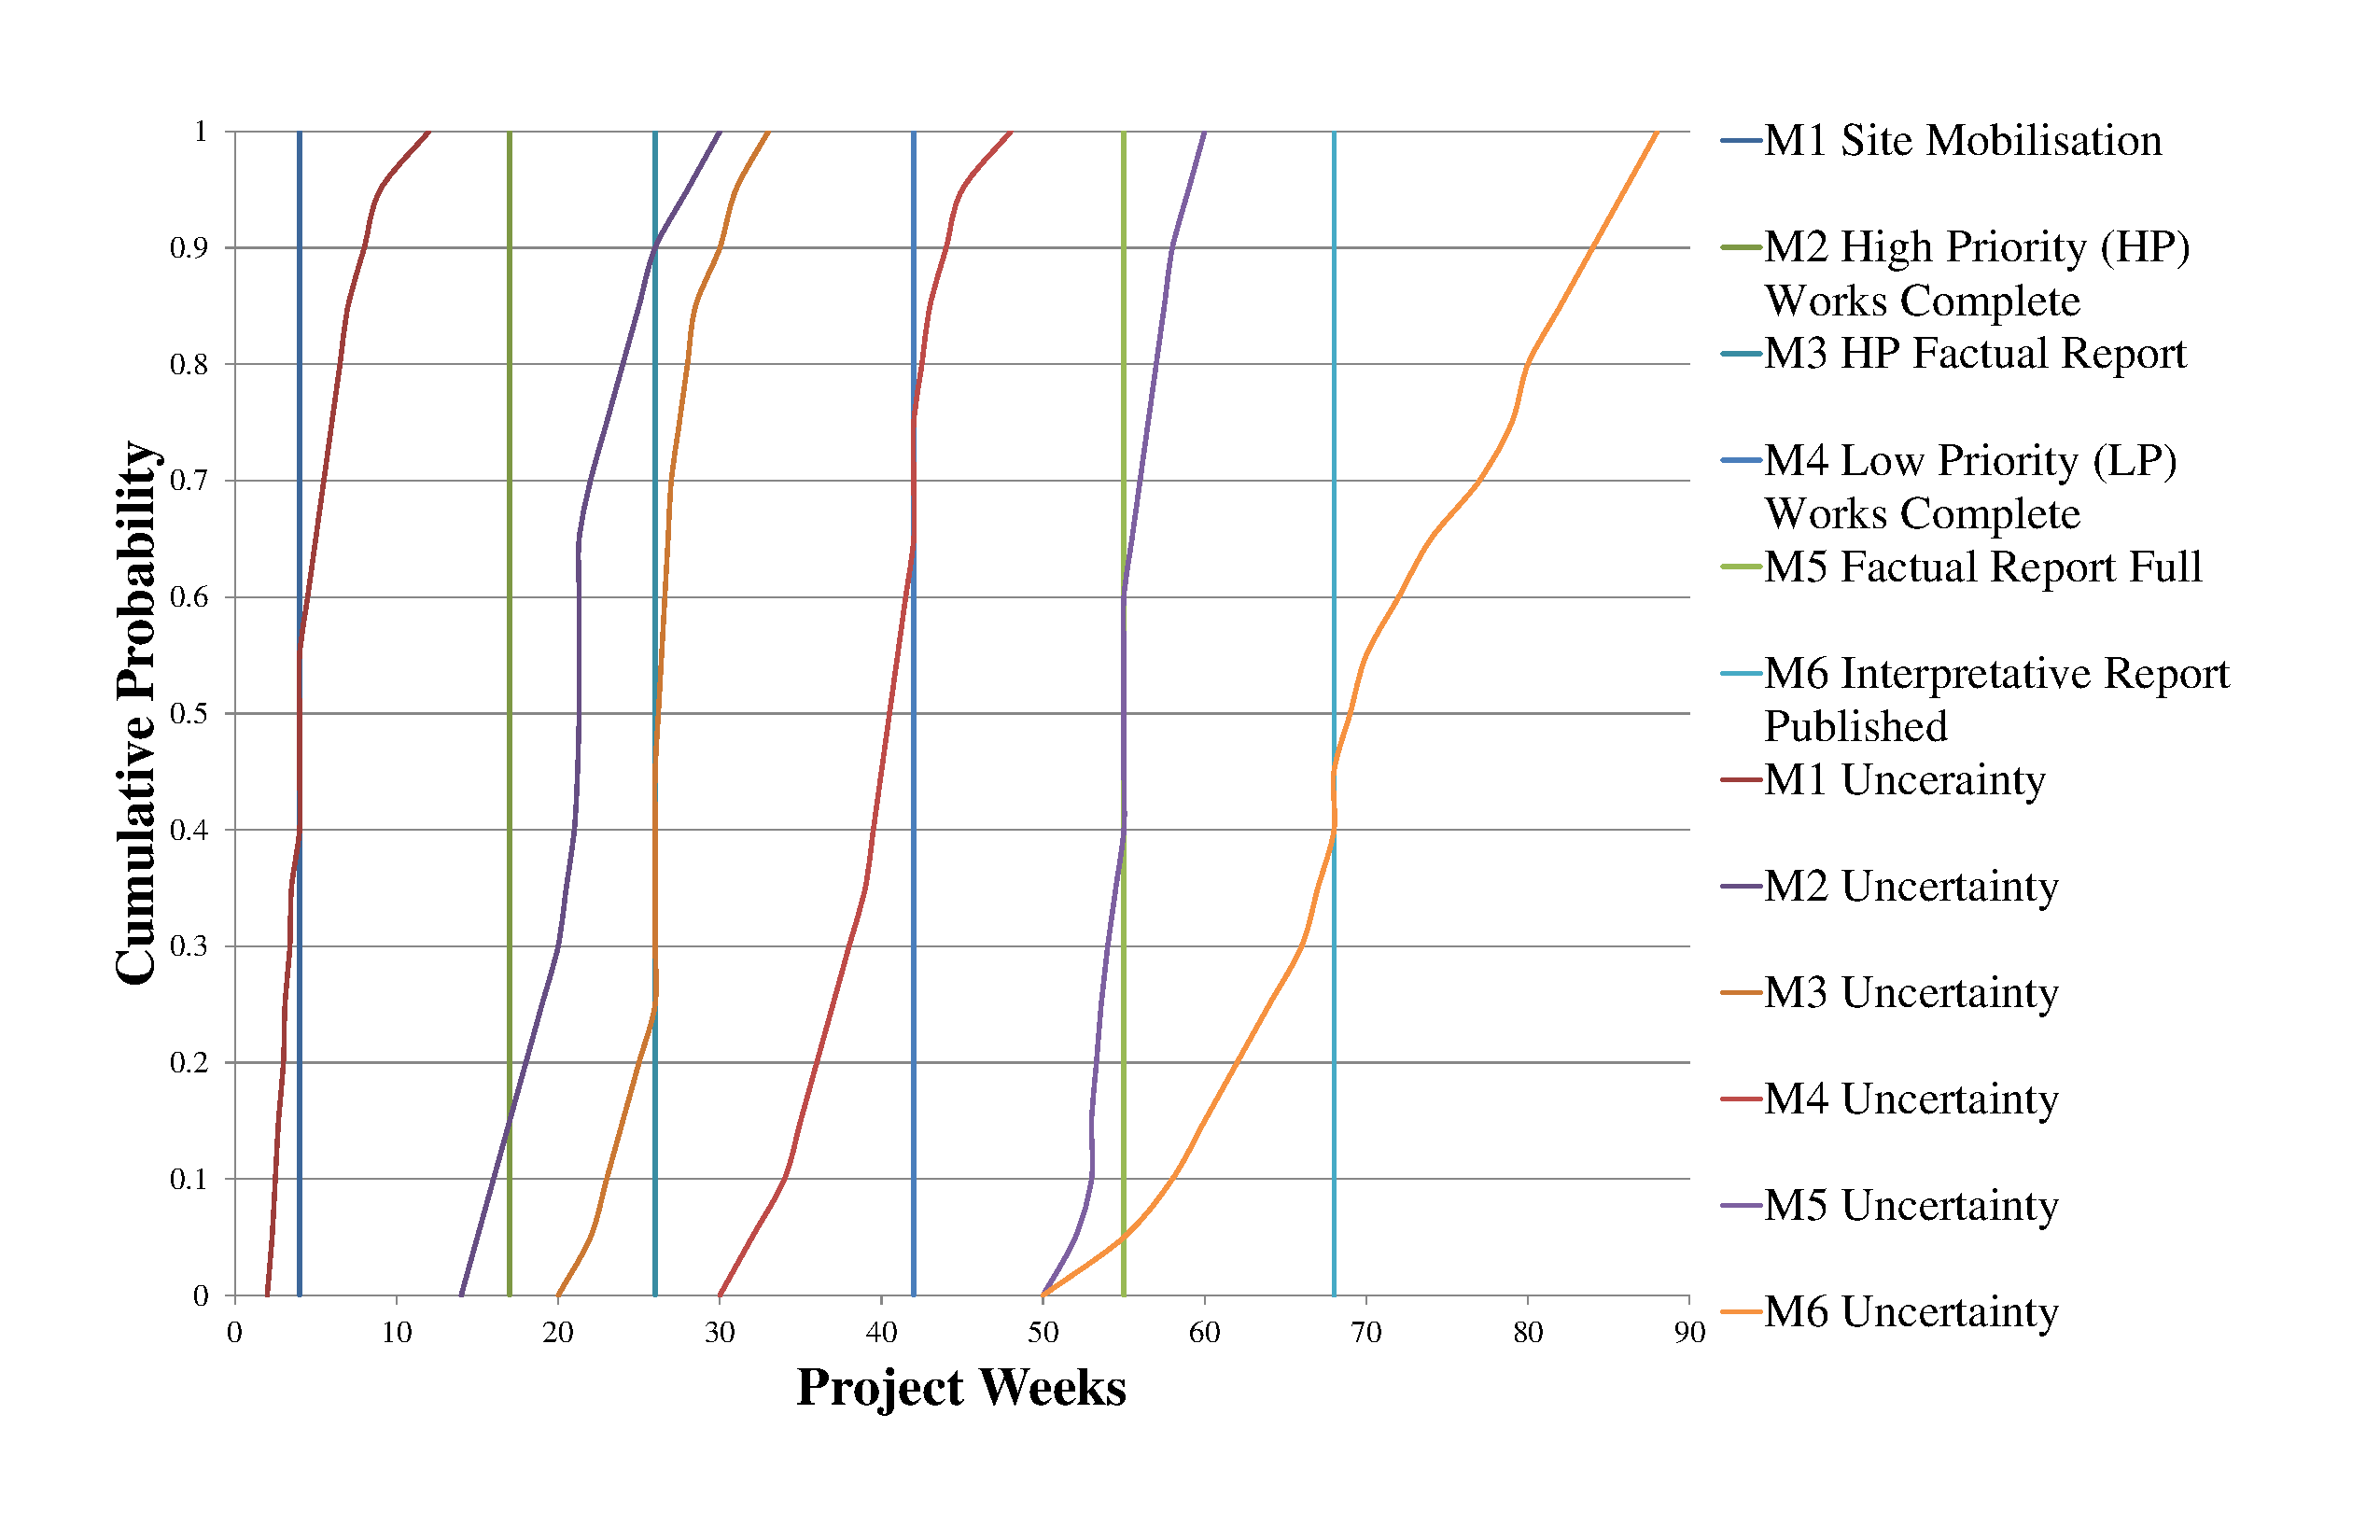
\includegraphics[width = 0.79\textwidth]{./Figures/ScheduleSensitivity.pdf} 
\caption{Schedule sensitivity diagram - adapted from \cite{hopkinson2008} \& \cite{chapman} }
\label{Figure:SensDiagGantt}
\end{figure}

There are alternative forms of sensitivity diagram which may be useful for presenting uncertainty when there are several different parameters involved. 
One of these is the tornado diagram, as shown in figure \ref{Figure:Tornado}, a common output from Monte Carlo simulation programs.
Each parameter is varied in turn whilst the others are held at a constant expected value.
The sources are then portrayed in order of significance.

\begin{figure}[!h]
  \centering
    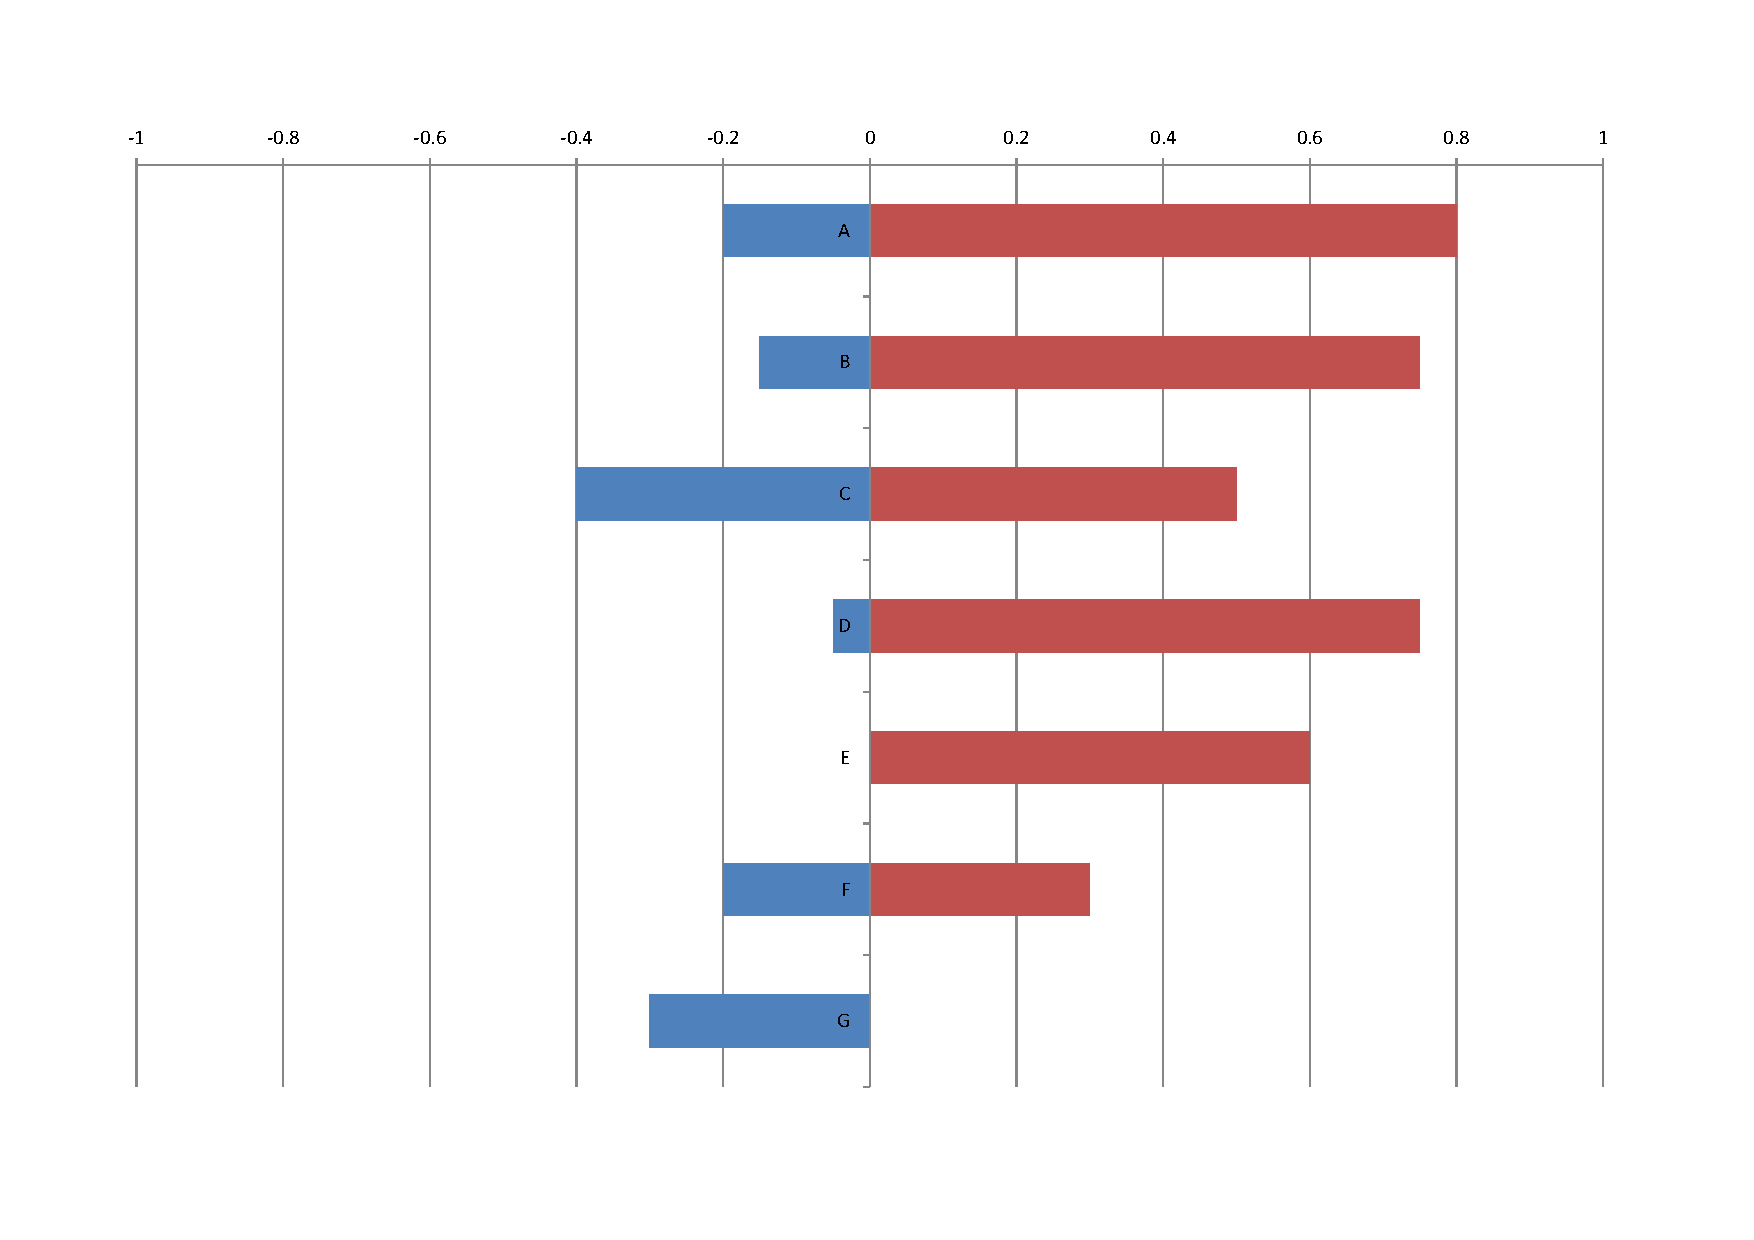
\includegraphics[width = 0.88\textwidth]{./Figures/TornadoFig.pdf} 
\caption{Tornado diagram - adapted from \cite{hopkinson2008}}
\label{Figure:Tornado}
\end{figure}

The evaluate phase is key to the successful implementation of an iterative process.
Iteration is one of the key sources of clarity efficiency which is harnessed through the PUMP approach and the reason for special focus on the evaluate phase in this report.
It is essential that on the first pass of the PUMP that only a rough sizing of all relevant sources is undertaken.
The aim is not to achieve an accurate probability estimate for all sources; this is not clarity efficient and means time is not spent optimally.
The first pass should result in a simple order-of-magnitude picture of the importance of the sources so that successive iterations can refine the most important sources where useful.

Informed, effective and efficient decision taking is the key deliverable so that opportunity efficiency can be maximised.
The evaluate phase consolidates the outputs from the other phases for presentation and interpretation.
Attention must be paid to how dependency and assumptions are dealt with during this phase.
Any analysis that does not adequately consider these factors should be discounted.
The use of a nested structure of sensitivity diagrams together with decision diagrams \citep{chapman} highlights the trade-offs between sources.
This interpretation of the portrayed uncertainty culminates in the effective shaping of base plans and project strategy so that risk inefficiency is minimised while opportunity efficiency is maximised.






\backmatter
\bibliographystyle{apalike}
\bibliography{ECS}


\appendix
%\appendixpage
%\appendixheaderon


\end{document}